\documentclass[a4paper,12pt]{article}

% Packages
\usepackage[utf8]{inputenc}
\usepackage[T1]{fontenc}
\usepackage[english]{babel}
\usepackage{amsmath,amsfonts,amssymb}
\usepackage{graphicx}
\usepackage{caption}
\usepackage{subcaption}
\usepackage{float}
\usepackage{cite}
\usepackage{hyperref}
\usepackage{geometry}

% Title and author
\title{ML Researcher Hands-On Challenge}
\author{Jibran Bohra}
\date{\today}

% Document start
\begin{document}

\maketitle

% Abstract
\begin{abstract}
This report provides a concise overview of the code development process, emphasizing the crucial functions and scripts involved. It serves as a comprehensive guide to the methodology adopted, facilitating a clear understanding of the implemented features and their respective outcomes.\end{abstract}

% Table of Contents
\tableofcontents
\newpage

% Sections
\section{Getting Started...}
\label{sec:introduction}
The provided \texttt{iPython} notebook served as the foundation for an Object-Oriented code development process. The resulting script, named \texttt{main.py}, is designed to preprocess an arbitrary dataset for utilization in a machine learning model. The key functions implemented in \texttt{main.py} are as follows:

\begin{itemize}
\item \texttt{generate\textunderscore features()}: This function reads structural data, including coordinates, occupancy, and $b$-factor, from \texttt{.pdb} files. The extracted information is then stored in \texttt{all\textunderscore data.json}.

\item \texttt{preprocess()}: This function gathers columns from \texttt{all\textunderscore data.json} for preprocessing. Specifically, it tokenizes protein sequence data, normalizes protein structure data (e.g., coordinates), and normalizes numerical data (e.g., coordinate mean and standard deviations, occupancy, $b$-factor). Additionally, class label data is prepared for one-hot encoding. The preprocessed data is saved in \texttt{structure.npy} and \texttt{preprocessed.json} for subsequent use.
\end{itemize}

\section{Methodology}
\label{sec:methodology}

The development process is thoroughly documented within the \texttt{development-process/} folder, housing scripts that illuminate significant milestones, including:

\begin{itemize}
\item \texttt{ann-labels}: An Artificial Neural Network (ANN) primarily employed as a sanity check. This ANN takes \textit{class} and \textit{architecture} as inputs, aiming to classify protein architecture. The model achieved $100\%$ accuracy, on par with expectations.
\item \texttt{ann-numerical}: An ANN dedicated to classifying protein architecture based on numerical data (as mentioned above). However, both training and validation accuracy were limited to approximately $\approx 25\%$.
\item \texttt{cnn-structure}: A Convolutional Neural Network (CNN) designed to derive correlative features from \texttt{structure.npy}, encompassing $x$-, $y$-, and $z$-coordinate data. Despite training accuracy generally being higher, validation accuracy plateaued at $\approx 20\%$, indicating a tendency to overfit, unlike \texttt{ann-numerical}.
\item \texttt{lstm-sequence}: A Long Short-Term Memory (LSTM) model utilized for processing tokenized protein sequence data. Model exhibited a capped validation accuracy of $\approx 20\%$ and a predisposition towards overfitting, much like \texttt{cnn-structure}.
\end{itemize}

\section{General Model and Results}
\label{sec:results}
Leveraging the advancements outlined earlier, a comprehensive model was constructed to classify protein architectures using protein sequence, protein structure, and various numerical data. The architecture of this model is highlighted in \texttt{all\textunderscore data \textunderscore classifier.py}. 


To enhance the dataset, data points were augmented by a factor of eight. Notably, structural and numerical data underwent systematic rescaling, while label and sequence data were straightforwardly replicated. The incorporation of data augmentation, along with the inclusion of dropout layers and regularization, aimed to alleviate tendencies toward overfitting. The training and validation performance of the general model over 1000 epochs is illustrated in Figure~\ref{fig:overall}.


\begin{figure}[h]
    \centering
    \begin{subfigure}[b]{0.45\textwidth}
        \centering
        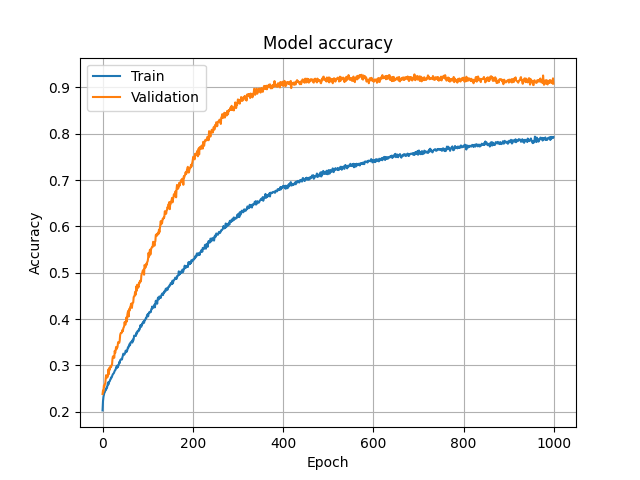
\includegraphics[width=\textwidth]{../training/model-accuracy.png}
        \caption{}
        \label{fig:subfig1}
    \end{subfigure}
    \hfill
    \begin{subfigure}[b]{0.45\textwidth}
        \centering
        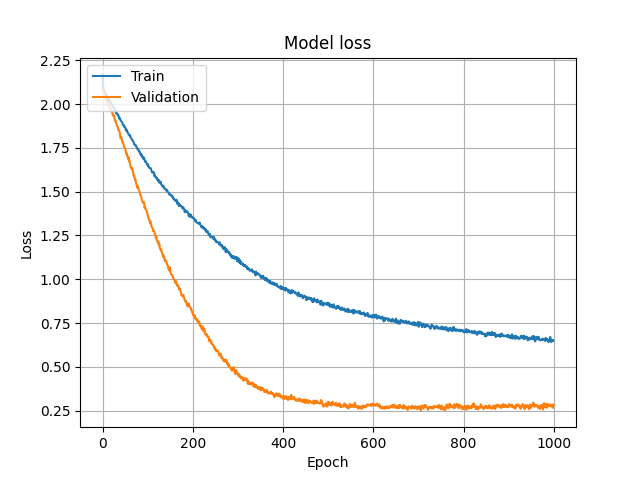
\includegraphics[width=\textwidth]{../training/model-loss.png}
        \caption{}
        \label{fig:subfig2}
    \end{subfigure}
    \caption{Model performance encapsulated by Figures~\ref{fig:subfig1}~and~\ref{fig:subfig2} demonstrates accuracy and loss, respectively,  across 1000 epochs}
    \label{fig:overall}
\end{figure}

Note that the relatively modest training performance can be attributed to the strategic use of dropout layers, which introduce random weight adjustments, coupled with the application of regularization techniques. Additionally, the validation accuracy levels off at around $\approx92\%$ during the 400$^{\text{th}}$ epoch, while the training accuracy continues to rise. This indicates that the peak model performance has been achieved and further training is likely to cause overfitting. 
\section{Discussion and Conclusion}
\label{sec:conclusion}
In conclusion, the general model crafted for the classification of protein architecture achieves an accuracy of $\approx90\%$ for unseen samples. To enhance performance and facilitate further development, it is advisable to employ a larger dataset. Additionally, it's crucial to acknowledge that the scope of this exercise was constrained by hardware limitations. I recommend training future models with a dedicated GPU to unlock greater computational capabilities and potentially improve outcomes.
% References
\begin{thebibliography}{99}
\bibitem{reference1}
Ronak Vijay,  \href{https://towardsdatascience.com/protein-sequence-classification-99c80d0ad2df}{\textit{Protein Sequence Classification: A case study on the Pfam dataset to classify protein families.}}
\end{thebibliography}
\end{document}
